\begin{table*}[t]
\centering
\begin{tabular}{p{0.15\linewidth}p{0.13\linewidth}p{0.13\linewidth}p{0.08\linewidth}p{0.08\linewidth}p{0.08\linewidth}p{0.08\linewidth}p{0.06\linewidth}}
\hline
Method & Resolution & Train Data & $J\&F_m$ & $J_m$ & $J_r$ & $F_m$ & $F_r$\\
\hline
Pretrained \cite{jabri2020walk} & 256 $\times$ 256 &  Kinetics & 72.74 & 73.92 & 74.76 & 71.56 & 69.56\\
\textbf{Ours} w/o normal & 640$\times$480 & ScanNet & 73.08 & 74.34 & \textbf{74.87} & 71.83 & 70.07 \\
\textbf{Ours} w/ normal & 640$\times$480 & ScanNet & \textbf{73.14} & \textbf{74.35} & 74.81 & \textbf{71.93} & \textbf{70.17} \\
\hline
\end{tabular}
 \vspace{-0.1in}
\caption{Video object segmentation results on ScanNet}
 \vspace{-0.15in}
\label{table:quan}
\end{table*}

% \vspace{+0.5in}



% \TODO{What is the data that you are using? What are the hyperparameters? How is the model evaluated? What are the baseline approaches that you are comparing your method with? How does the performance of your method compare with these baseline methods? Tables and figures are efficient ways to convey your experiment results.}
\subsection{Dataset}
\begin{figure*}[!t]
    \centering
    \resizebox{1.0\textwidth}{!}{
    \begin{tabular}{ccccccccc}
    \toprule
    w/o normal
    &\frame{\includegraphics[width=0.15\textwidth]{example_wall/e01_no_normal/0_0_blend.jpg}} 
    &\frame{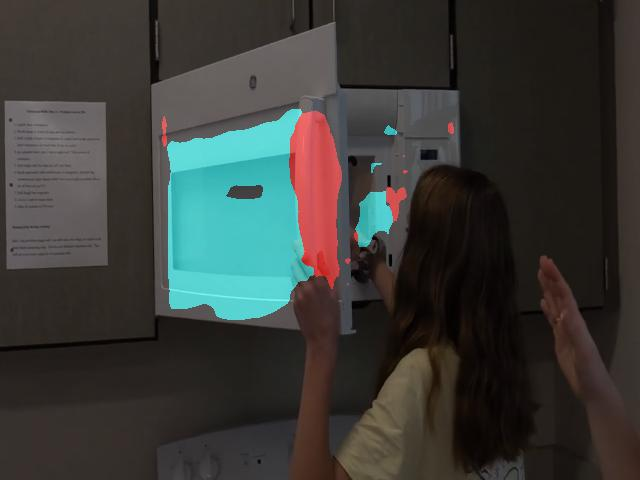
\includegraphics[width=0.15\textwidth]{example_wall/e01_no_normal/0_1_blend.jpg}}
    &\frame{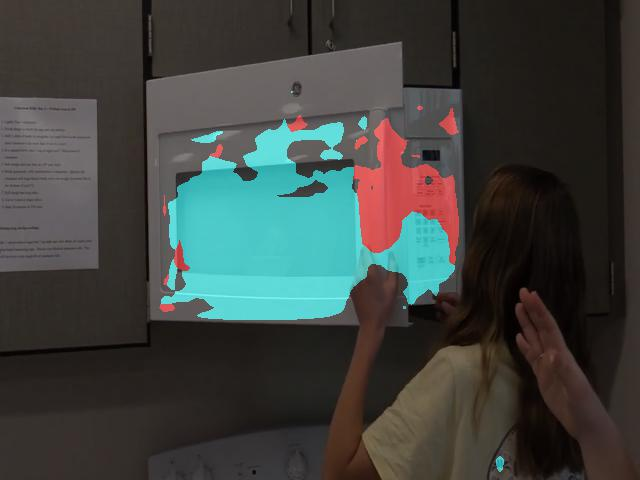
\includegraphics[width=0.15\textwidth]{example_wall/e01_no_normal/0_2_blend.jpg}} 
    &\frame{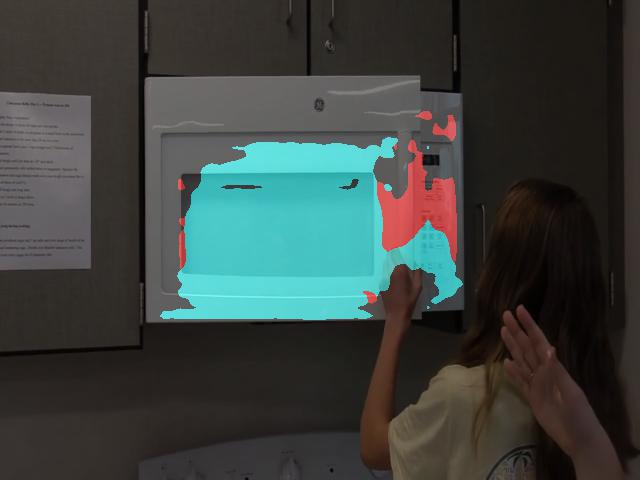
\includegraphics[width=0.15\textwidth]{example_wall/e01_no_normal/0_3_blend.jpg}}
    &\frame{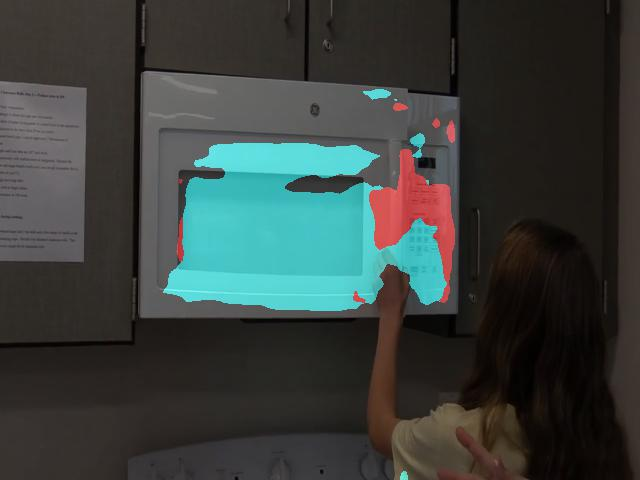
\includegraphics[width=0.15\textwidth]{example_wall/e01_no_normal/0_4_blend.jpg}} 
    &\frame{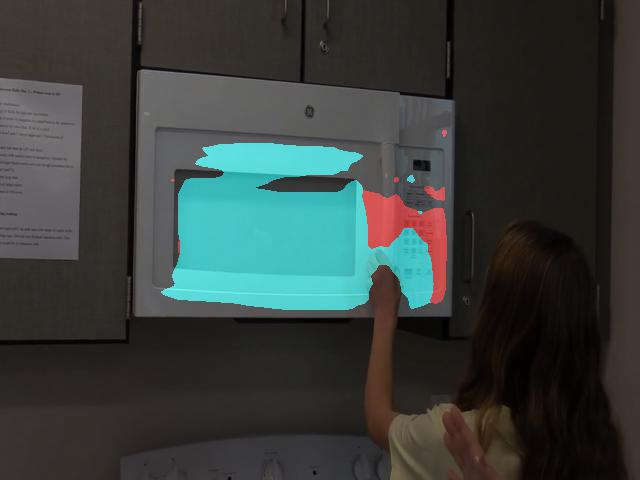
\includegraphics[width=0.15\textwidth]{example_wall/e01_no_normal/0_5_blend.jpg}}
    &\frame{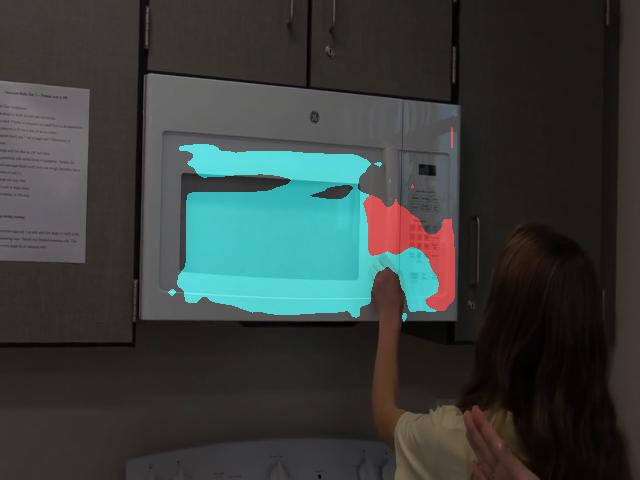
\includegraphics[width=0.15\textwidth]{example_wall/e01_no_normal/0_6_blend.jpg}} 
    &\frame{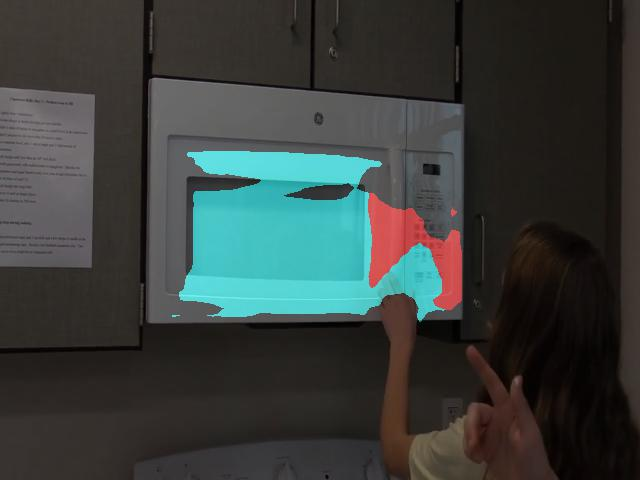
\includegraphics[width=0.15\textwidth]{example_wall/e01_no_normal/0_7_blend.jpg}} \\
    
    w/ normal
    &\frame{\includegraphics[width=0.15\textwidth]{example_wall/e01_ours/0_0_blend.jpg}} 
    &\frame{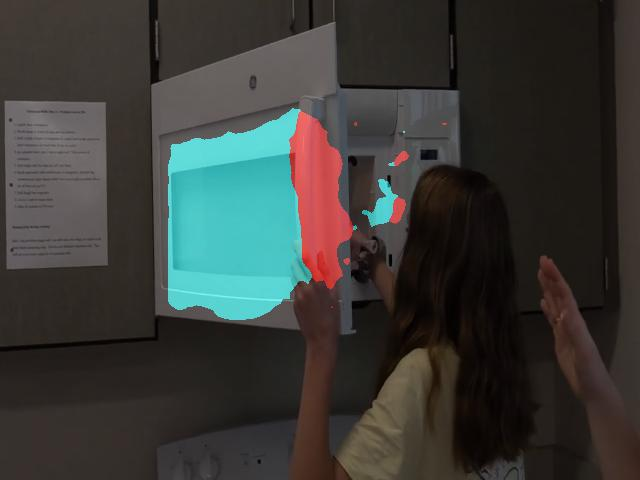
\includegraphics[width=0.15\textwidth]{example_wall/e01_ours/0_1_blend.jpg}}
    &\frame{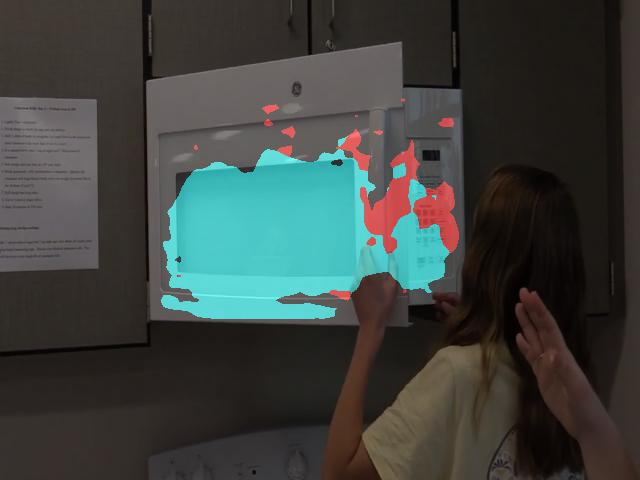
\includegraphics[width=0.15\textwidth]{example_wall/e01_ours/0_2_blend.jpg}} 
    &\frame{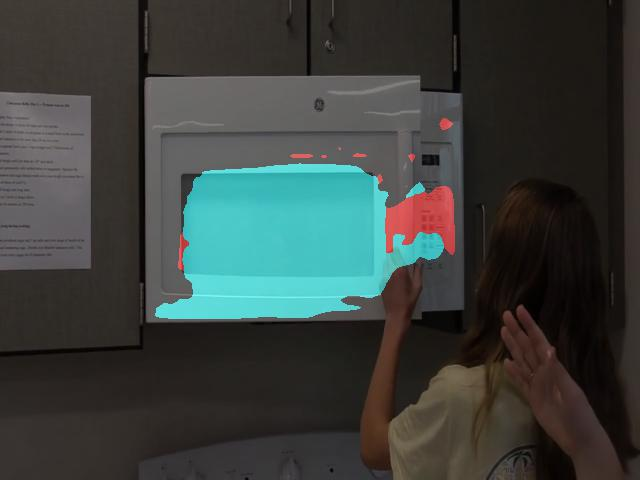
\includegraphics[width=0.15\textwidth]{example_wall/e01_ours/0_3_blend.jpg}}
    &\frame{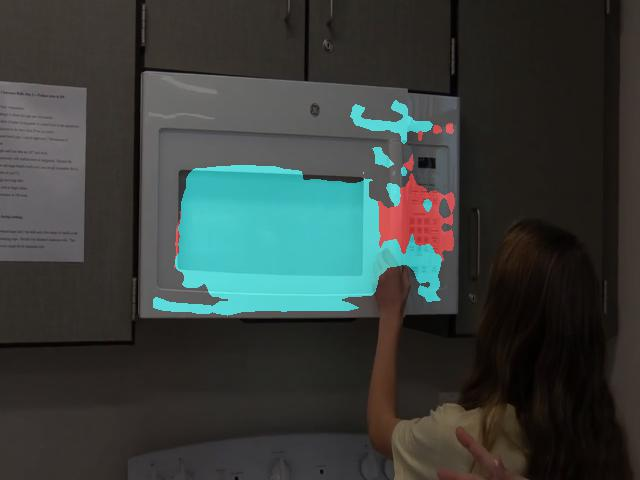
\includegraphics[width=0.15\textwidth]{example_wall/e01_ours/0_4_blend.jpg}} 
    &\frame{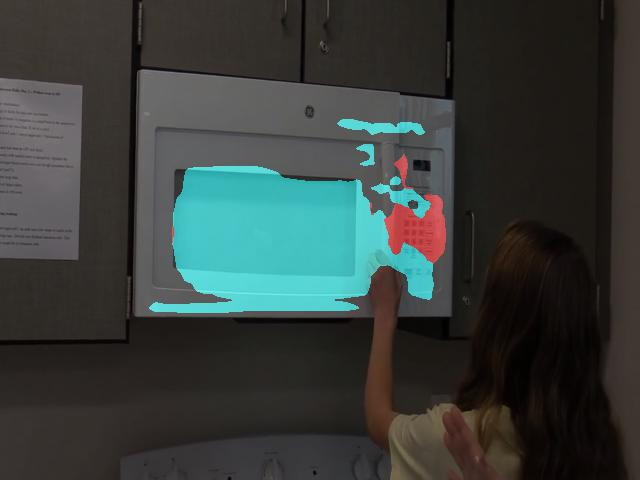
\includegraphics[width=0.15\textwidth]{example_wall/e01_ours/0_5_blend.jpg}}
    &\frame{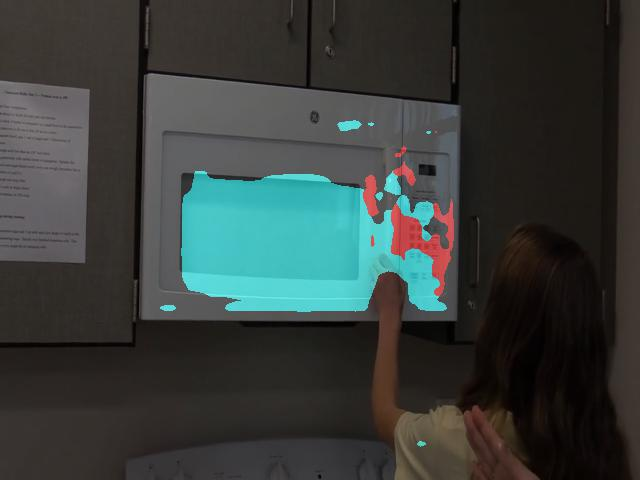
\includegraphics[width=0.15\textwidth]{example_wall/e01_ours/0_6_blend.jpg}} 
    &\frame{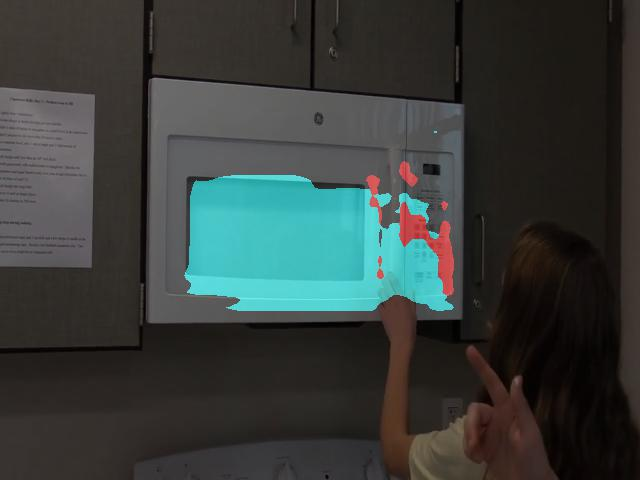
\includegraphics[width=0.15\textwidth]{example_wall/e01_ours/0_7_blend.jpg}} \\
    
    ~\cite{jabri2020walk} pretrained
    &\frame{\includegraphics[width=0.15\textwidth]{example_wall/e01_pretrained/0_0_blend.jpg}} 
    &\frame{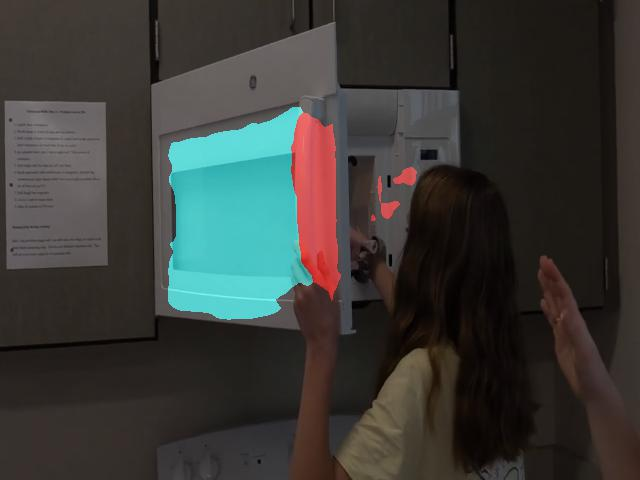
\includegraphics[width=0.15\textwidth]{example_wall/e01_pretrained/0_1_blend.jpg}}
    &\frame{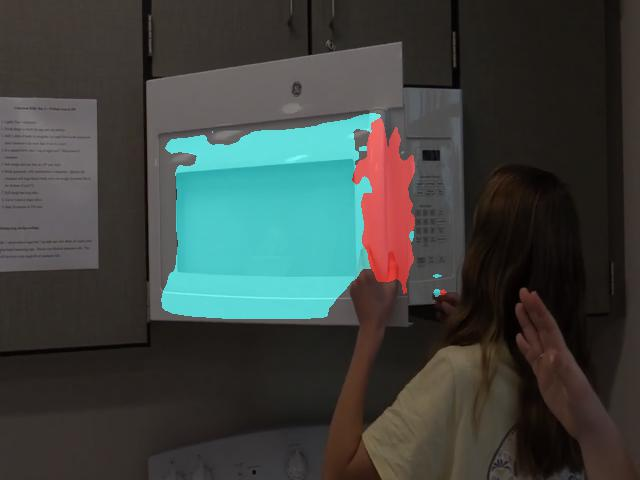
\includegraphics[width=0.15\textwidth]{example_wall/e01_pretrained/0_2_blend.jpg}} 
    &\frame{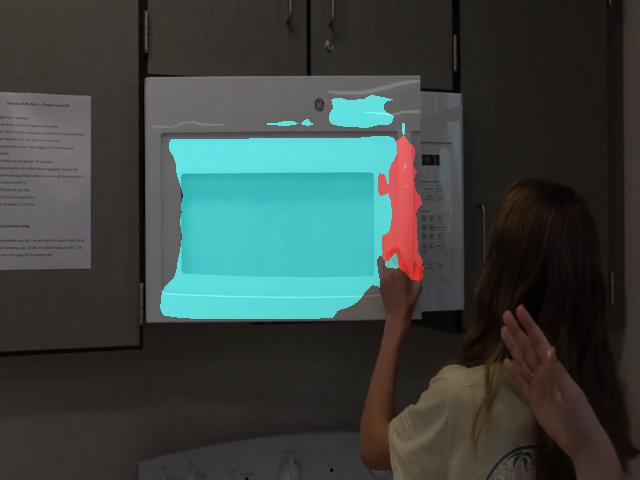
\includegraphics[width=0.15\textwidth]{example_wall/e01_pretrained/0_3_blend.jpg}}
    &\frame{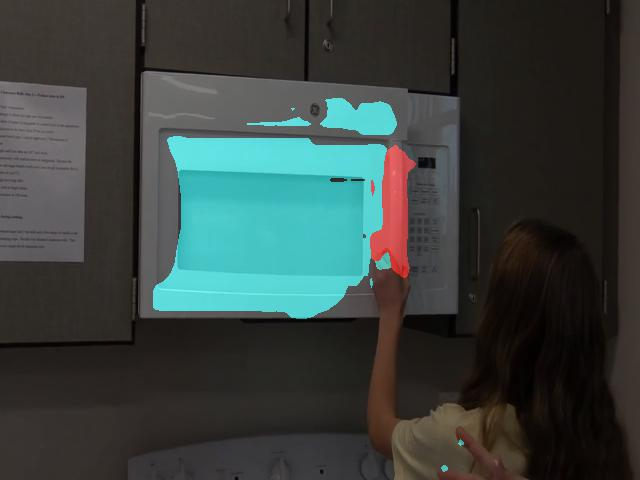
\includegraphics[width=0.15\textwidth]{example_wall/e01_pretrained/0_4_blend.jpg}} 
    &\frame{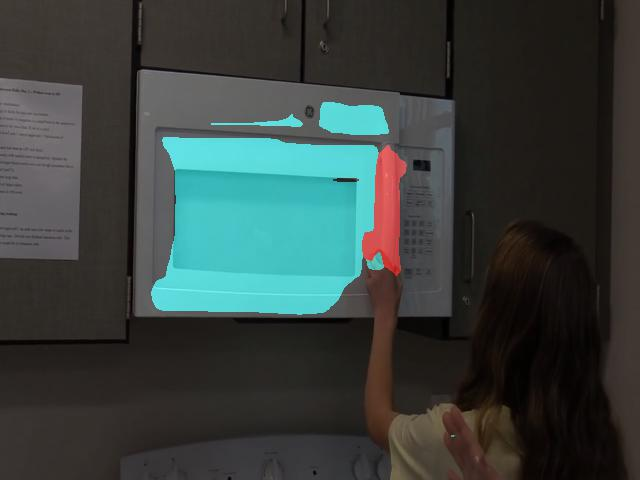
\includegraphics[width=0.15\textwidth]{example_wall/e01_pretrained/0_5_blend.jpg}}
    &\frame{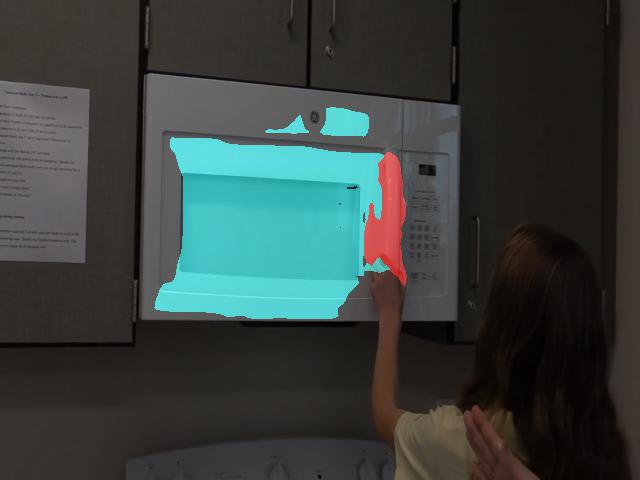
\includegraphics[width=0.15\textwidth]{example_wall/e01_pretrained/0_6_blend.jpg}} 
    &\frame{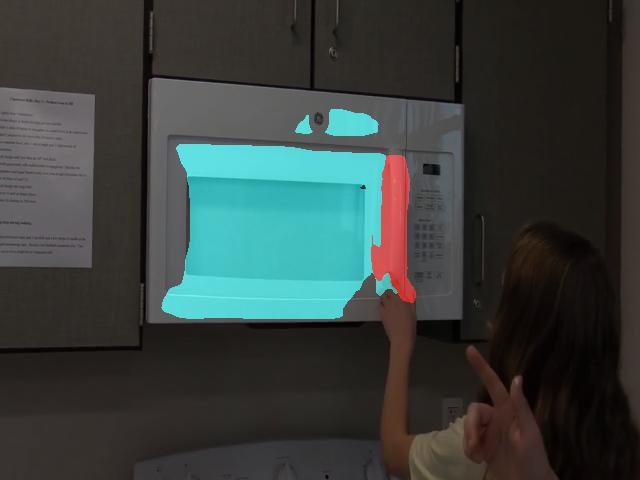
\includegraphics[width=0.15\textwidth]{example_wall/e01_pretrained/0_7_blend.jpg}} \\
    \bottomrule
    \end{tabular}
    }
    \vspace{-0.1in}
    
    \caption{Qualitative results on videos with dynamic scene of the label propagation task given an initial plane detection from PlaneRCNN model.}
    \label{fig:dynamic}
    \vspace{-0.2in}
\end{figure*}
%  dataset containing 2.5 million views in more than 1500 scans, annotated with 3D camera poses, surface reconstructions, and instance-level semantic segmentations.
We use ScanNet \cite{dai2017scannet} to train and evaluate our model for tracking 3D planes. ScanNet \cite{dai2017scannet} is an indoor RGB-D video dataset with surface reconstructions and instance segmentation annotations. The instance indices are consistent throughout the video frames which enables the evaluation for 3D object tracking. We downsample the image resolution from 1296 $\times$ 968 to 640 $\times$ 480 using bilinear interpolation. The instance masks are resized with the same ratio except that the nearest-neighbour interpolation is used to avoid introducing new instance indices. We use 10 scenes for training and 2 scenes for testing. Each scene contains 1000 to 5000 frames. See Figure \ref{fig:impair} and \ref{fig:mesh} for illustrations.


\subsection{Evaluation Metric}

We follow \cite{jabri2020walk} and two complementary criteria are employed to measure how our mask prediction $M$ fits the ground truth mask $G$. 

\par \noindent {\bf Region Similarity $\boldsymbol{J}$.} To measure the region-based segmentation similarity, the commonly used metric IoU (intersection-over-union, also known as the Jaccard index) is used. $J$ can be calculated as $J = \left| \frac{M \cap G}{M \cup G} \right|$.



\par \noindent {\bf Contour Accuracy $\boldsymbol{F}$.} Precision $P_c$ and recall $R_c$ can be calculated based on the contours extracted from $M$ and $G$. Then the F-measure $F$ can be calculated as $F = \frac{2P_cR_c}{P_c + R_c}$ to achieve a good trade-off between the two.

We follow \cite{jabri2020walk} to report mean (m) and recall (r) of the region similarity ($J$) and boundary alignment ($F$) \cite{perazzi2016benchmark}.


\begin{figure}[H]
  \centering
  \begin{subfigure}[b]{0.4\columnwidth}
    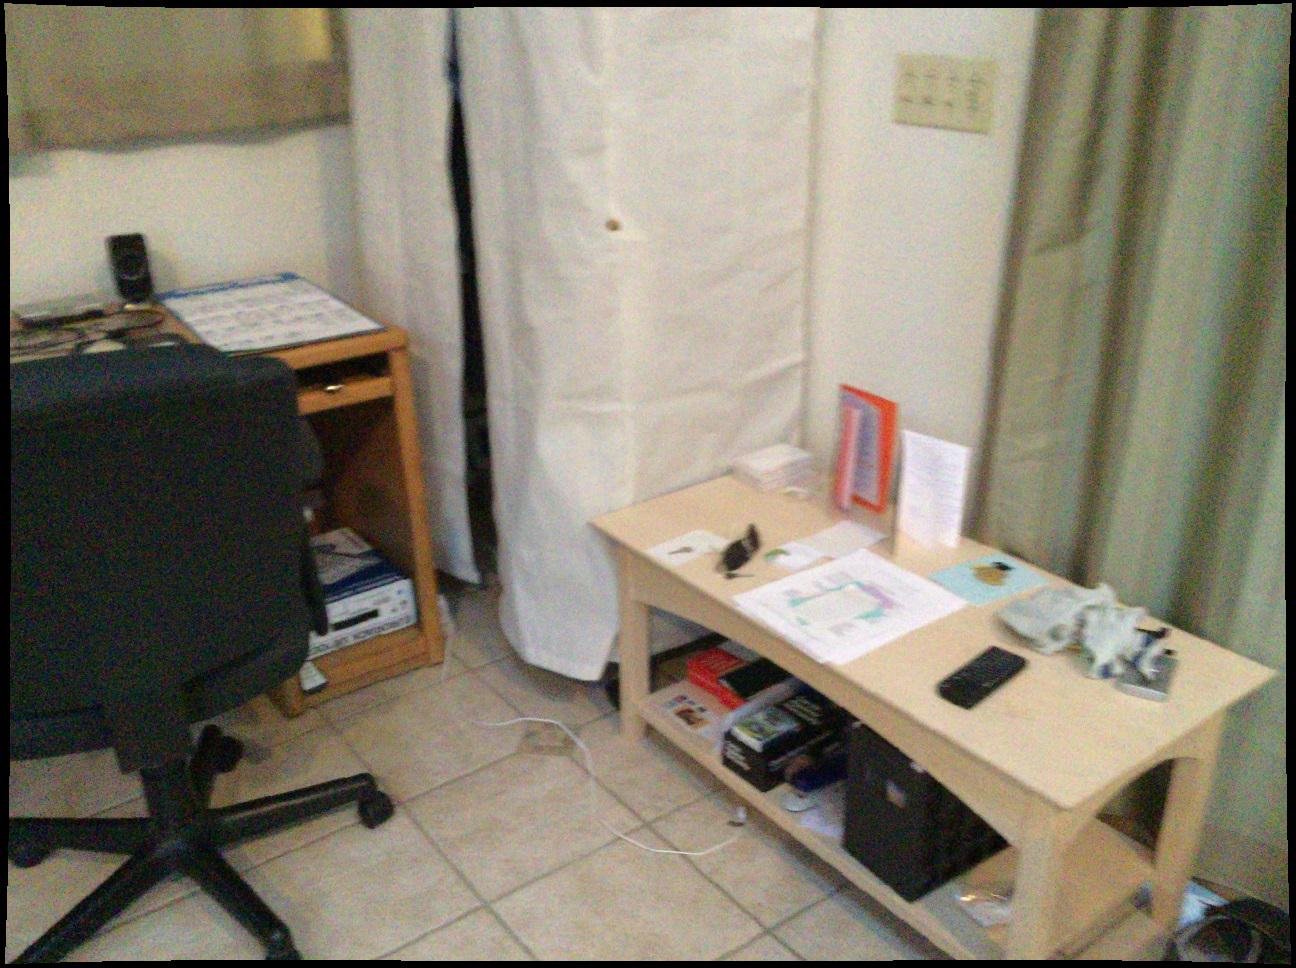
\includegraphics[width=\linewidth]{FinalReport/dataset_example/original.jpg}
    \caption{Scene Example}
  \end{subfigure}
  \begin{subfigure}[b]{0.4\columnwidth}
    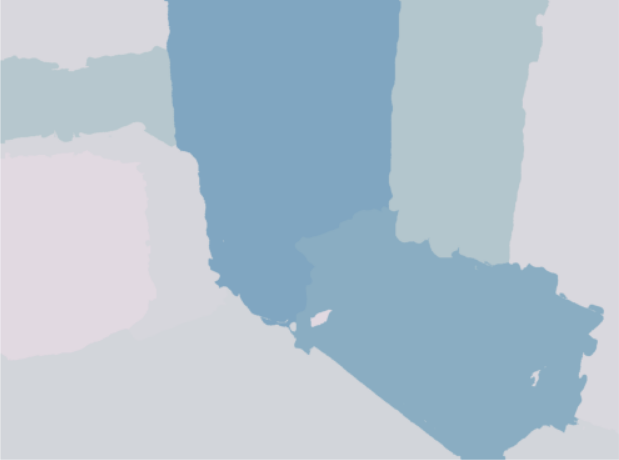
\includegraphics[width=\linewidth]{FinalReport/dataset_example/4.png}
    \caption{Instance Segmentation}
  \end{subfigure}
  \vspace{-0.1in}
  \caption{Image Mask Pair \cite{dai2017scannet}}
  \label{fig:impair}
      \vspace{-0.2in}
\end{figure}


% \vspace{-0.1in}
\begin{figure}[H]
  \centering
  \begin{subfigure}[b]{0.44\columnwidth}
    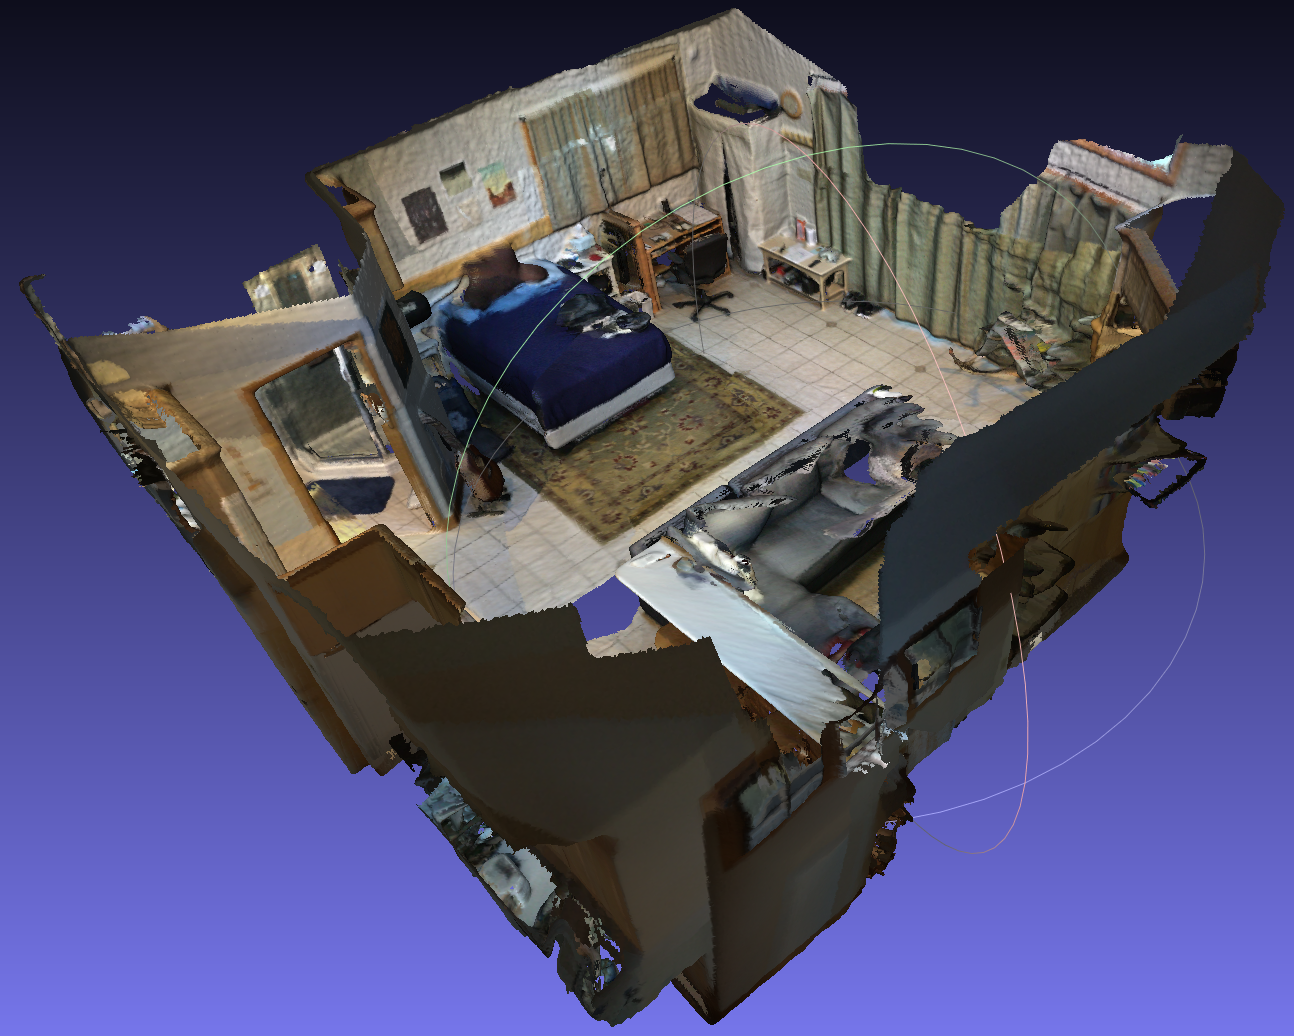
\includegraphics[width=\linewidth]{FinalReport/dataset_example/scene_mesh.png}
    \caption{Surface Reconstruction}

  \end{subfigure}
  \begin{subfigure}[b]{0.41\columnwidth}
    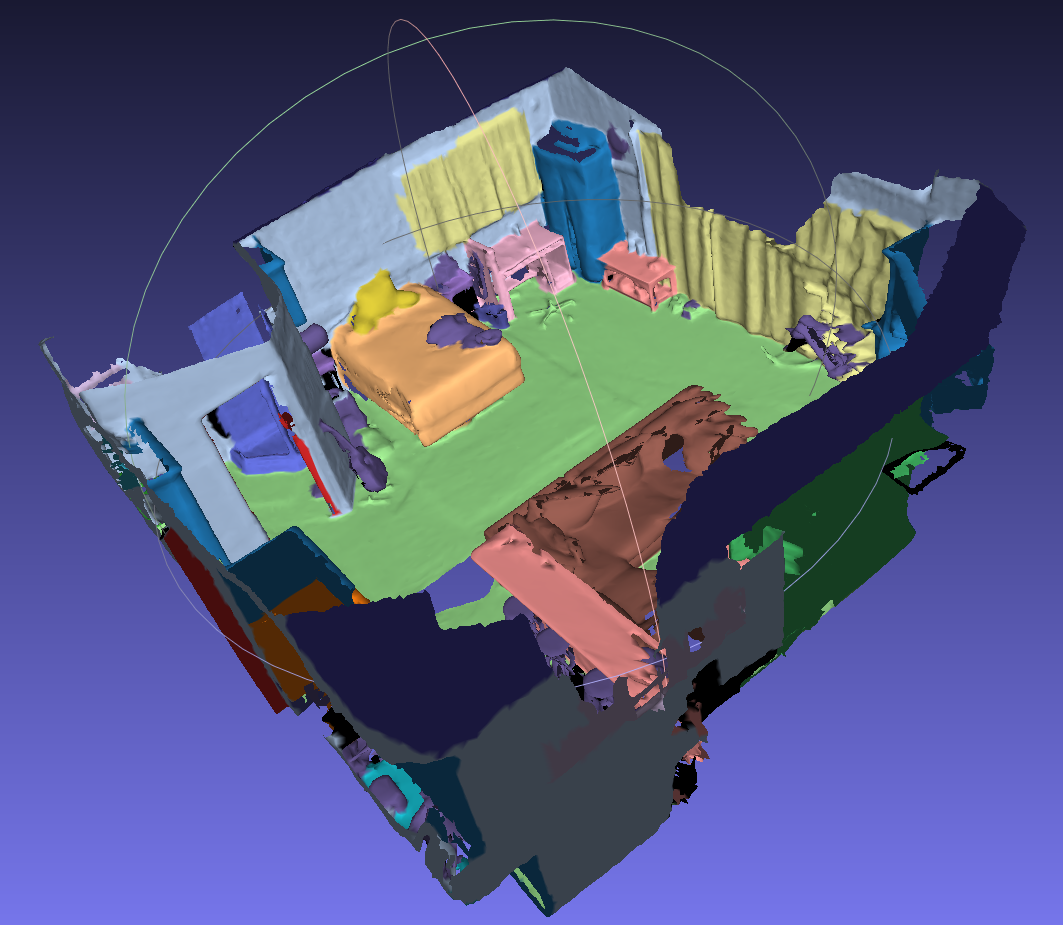
\includegraphics[width=\linewidth]{FinalReport/dataset_example/scene_label.png}
    \caption{Labeled Mesh}
  \end{subfigure}
    \vspace{-0.1in}
  \caption{Mesh Model \cite{dai2017scannet}}
      \vspace{-0.25in}
  \label{fig:mesh}
\end{figure}




\par \noindent {\bf Baselines.} We use two baseline models to compare with our proposed method. All models share the same network architecture. The first baseline is the pretrained model provided by \cite{jabri2020walk}, which only uses the self-supervised palindrome loss and is trained on the Kinetics400 \cite{carreira2017quo}. The second baseline is trained on a subset of the ScanNet scenes from scratch but without considering the surface normal constraints in the affinity matrix and the random-walk loss. Our model in contrast, is trained on the same subset of ScanNet from scratch and takes the normal difference into consideration as described in section \ref{sec:method}.

% \vspace{-0.2in}
\begin{figure}[H]
  \centering
  \begin{subfigure}[b]{0.85\columnwidth}
    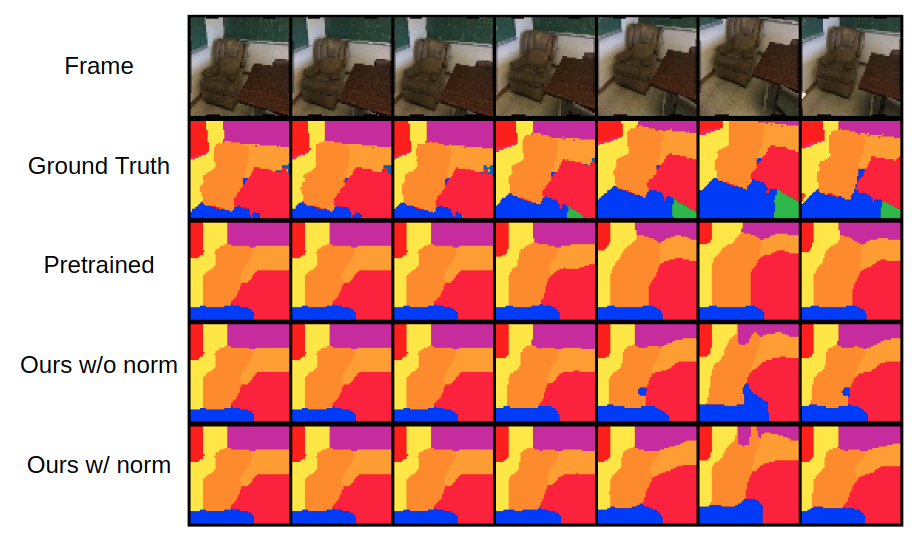
\includegraphics[width=\linewidth]{FinalReport/dataset_example/gt0030.png}
    \caption{Test scene A}
  \end{subfigure}
  \begin{subfigure}[b]{0.85\columnwidth}
    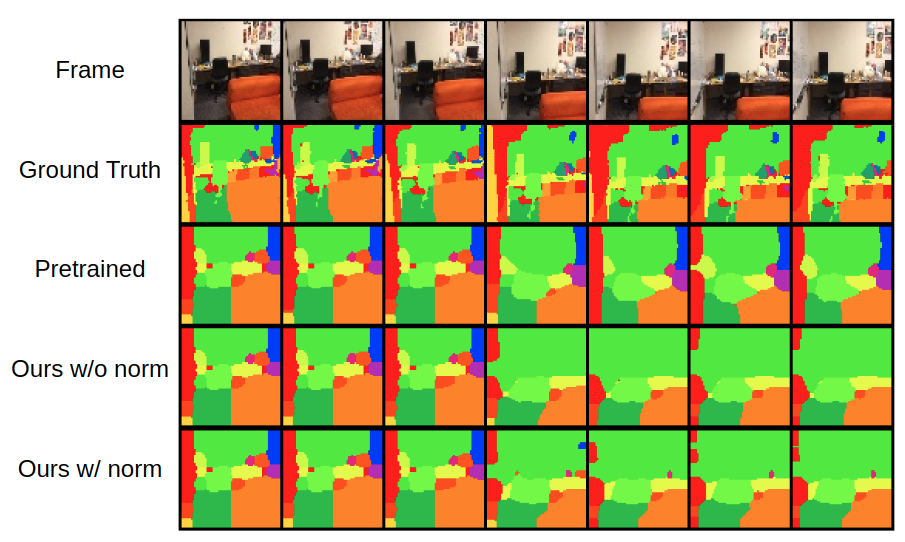
\includegraphics[width=\linewidth]{FinalReport/dataset_example/gt0040.png}
    \caption{Test scene B}
  \end{subfigure}
  \vspace{-0.1in}
  \caption{Test Scenes}
    \vspace{-0.3in}
  \label{fig:video_seg}
\end{figure}

\vspace{-0.05in}
% \titlespacing*{\subsection}{0pt}

\subsection{Qualitative Results}

We present some inference results from the two baseline models as well as our model, see Figure \ref{fig:video_seg}. The inference results are the instance segmentation masks of the scene, where the instance indices are consistent throughout the frames. We select two new scenes from the ScanNet dataset that are different from the training data in order to test the generalization ability of our model. 

% \TODO{interpretation here}
As shown in Figure \ref{fig:video_seg} a, our model with normal constraints can have denoising and smoothing effects on the plane detection (e.g. 5th column) compared with the model without normal constraints. However, it can also be subject to noises. As can be observed in Figure \ref{fig:video_seg} b, a small object with regional salient normal can induce noisy plane detection compared to the pretrained model (e.g. 7th column).

%\ref{fig:dynamic}
We also evaluate the methods on a dynamic scene, and the results are shown in Figure \ref{fig:dynamic}. All the three methods cannot predict the planes for the door and the handle perfectly, underlining the improvement space for our model on dynamic scenes.

\subsection{Quantitative Results}
Our quantitative results are listed in table \ref{table:quan}. Unsurprisingly, our model trained on the ScanNet \cite{dai2017scannet} outperforms the pretrained model \cite{jabri2020walk} on the test scenes because of the data distribution similarity. Our model with normal constraints slightly improves the model without normal constraints with limited training. This approach is promising if more training resources are available.
